\subsection{User Management}
This module is responsible for reading data from the client user database. It will do this by making use of ldap.js .
\subsubsection{Scope}
\paragraph{Test}
\subsubsection{Use cases}
\begin{itemize}
\item Autorize
\item validateUserName
\item retrieveEmail
\end{itemize}
\subsubsection{Domain model}
\subsection{Project}
\subsubsection{Scope}
\subsubsection{Use cases}
\subsubsection{Domain model}
\subsection{Estimation}
\subsubsection{Scope}
\subsubsection{Use cases}
\subsubsection{Domain model}
\subsection{Report}
\subsubsection{Scope}
\subsubsection{Use cases}
\subsubsection{Domain model}
\subsection{Notification}
\subsubsection{Scope}
This is the notification scope
	\begin{figure}[H]
	    	\centering
	    	\fbox{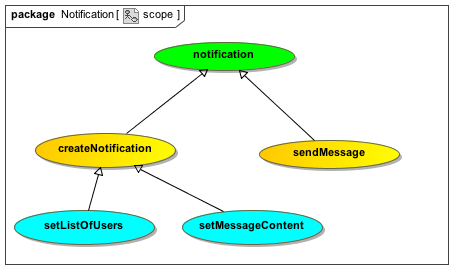
\includegraphics[width=0.5\textwidth]{Notification_Scope}}
	    	\caption{Notifications Scope}
	    	\label{fig:Notification_Scope}
   	\end{figure}
\subsubsection{Use cases}
\subsubsection{Domain model}
